\documentclass[]{article}

\usepackage{cite} % Add this line to include the cite package
% \usepackage[backref]{hyperref} % Add this line to include the hyperref package

\usepackage{amsmath} % Add this line to include the amsmath package
\usepackage{graphicx} % Add this line to include the graphicx package
\usepackage{fancyhdr}

\title{\textbf{Computer Vision homework 2}}
\author{Pan Changxun}
\date{March 2025}

\topmargin=-0.45in      %
\evensidemargin=0in     %
\oddsidemargin=0in      %
\textwidth=6.5in   
\textheight=9.0in       %
\headsep=0.25in 

\pagestyle{fancy}
\fancyhf{} % Clear all header and footer fields
\fancyhead[L]{Pan Changxun} % Left header
\fancyhead[C]{Computer Vision homework 2} % Center header
\fancyhead[R]{March 2025} % Right header
%\fancyfoot[L]{\leftmark} % Left footer
\fancyfoot[C]{\thepage} % Center footer
%\fancyfoot[R]{} % Right footer

\begin{document}
\maketitle

\section{3D Location Transformation}
\begin{enumerate}
	\item[a)] The intrinsic matrix is given by:
	\begin{equation}
		K = \begin{bmatrix}
			f_x & 0 & c_x \\
			0 & f_y & c_y \\
			0 & 0 & 1
		\end{bmatrix}
	\end{equation}
	When \(f_x = f_y = f = 721.5mm\) and \(c_x, c_y = (609.6, 172.9)mm\), the intrinsic matrix becomes:
	\begin{equation}
		K = \begin{bmatrix}
			721.5 & 0 & 609.6 \\
			0 & 721.5 & 172.9 \\
			0 & 0 & 1
		\end{bmatrix}
	\end{equation}
	\item[b)] The equation of the ground plane in camera's coordinate system is \(y=1.7m\).
	\item[c)] When given a 2D point (x,y) in the image and suppose it lies on the ground (y=1.7m), we can find the corresponding 3D point in the camera's coordinate system using the following equations:
	\begin{equation}
		Y = 1.7m
	\end{equation}
	\begin{equation}
		Z = \frac{Y \cdot f_y}{y - c_y} = \frac{1.7m \cdot 721.5mm}{y - 172.9mm}
	\end{equation}
	\begin{equation}
		X = Y \cdot \frac{x - c_x}{y - c_y} = 1.7m \cdot \frac{x - 609.6mm}{y - 172.9mm}
	\end{equation}
	where (X, Y, Z) are the coordinates of the corresponding 3D point in the camera's coordinate system and \(c_x, c_y\) equals to (609.6, 172.9)mm.
\end{enumerate}

\section{Road Analyzing}
\begin{enumerate}
	\item[a)] The depth maps are stored in the folder "/src/problem2\_analyzing/data/depth/" with corresponding colorbar. Here is an example of the depth map:
	\begin{figure}[h]
		\centering
		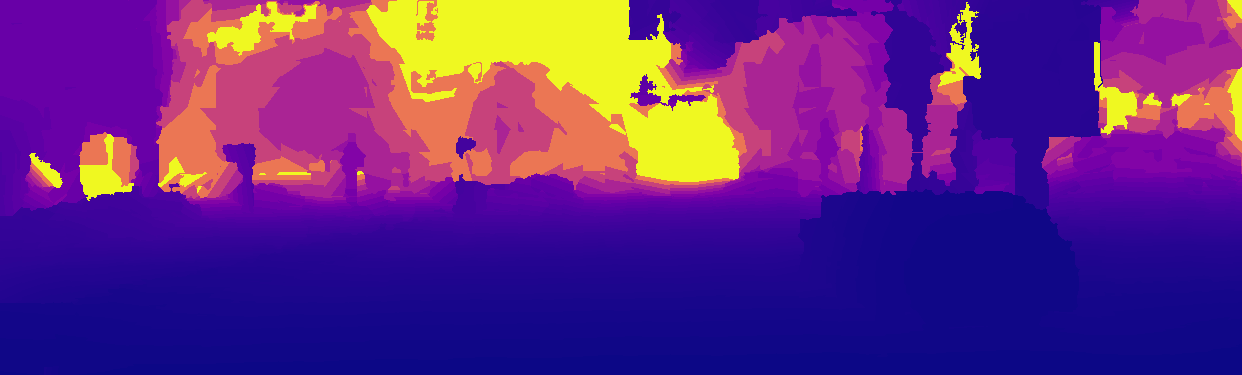
\includegraphics[width=0.5\textwidth]{src/problem2_analyzing/data/depth/004945_depth.png}
		\caption{004945\_depth map}
		\label{fig:depth_map_example}
	\end{figure}
	\newpage
	And here is the colorbar for the depth map:
	\begin{figure}[h]
		\centering
		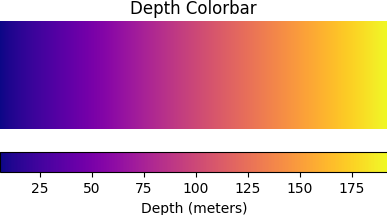
\includegraphics[width=0.5\textwidth]{src/problem2_analyzing/data/depth/004945_colorbar.png}
		\caption{004945\_depth map colorbar}
		\label{fig:colorbar}
	\end{figure}
	\item[b)] Visualize the bounding boxes in the images are stored in the folder "/src/problem2\_analyzing/data/bbox/". Here is an example of the bounding box visualization:
	\begin{figure}[h]
		\centering
		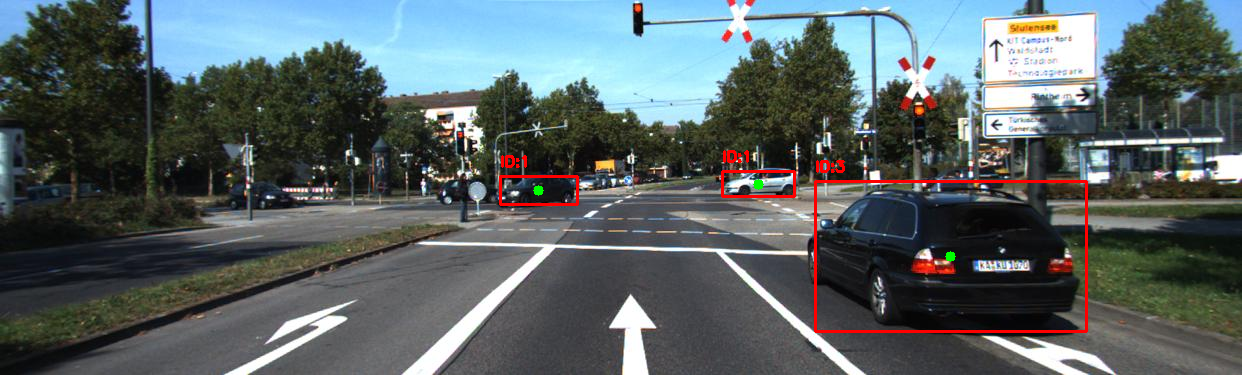
\includegraphics[width=0.5\textwidth]{src/problem2_analyzing/data/bbox/004945_bbox.png}
		\caption{004945 bounding box visualization}
		\label{fig:bbox_visualization}
	\end{figure}
	And the 3D coordinates of the center of the bounding box are stored in the folder "/src/problem2\_analyzing/data/3d\_coordinates/". Here are examples of the 3D coordinates of 004945:
		\begin{enumerate}
			\item ID: 3, original 2D coordinates: [950 256], 3D Coordinates: [3.2385147  0.79094404 6.863781  ]
			\item ID: 1, original 2D coordinates: [758 184], 3D Coordinates: [ 9.884517   0.7422009 48.046467 ]
			\item ID: 1, original 2D coordinates: [538 190], 3D Coordinates: [-3.4654994  0.8303526 34.942886 ]
		\end{enumerate}
\end{enumerate}

\newpage
\section{Self-driving Detection (Bonus)}
Here are the keypoints of the self-driving detection algorithm:
% two figures
\begin{figure}[h]
	\centering
	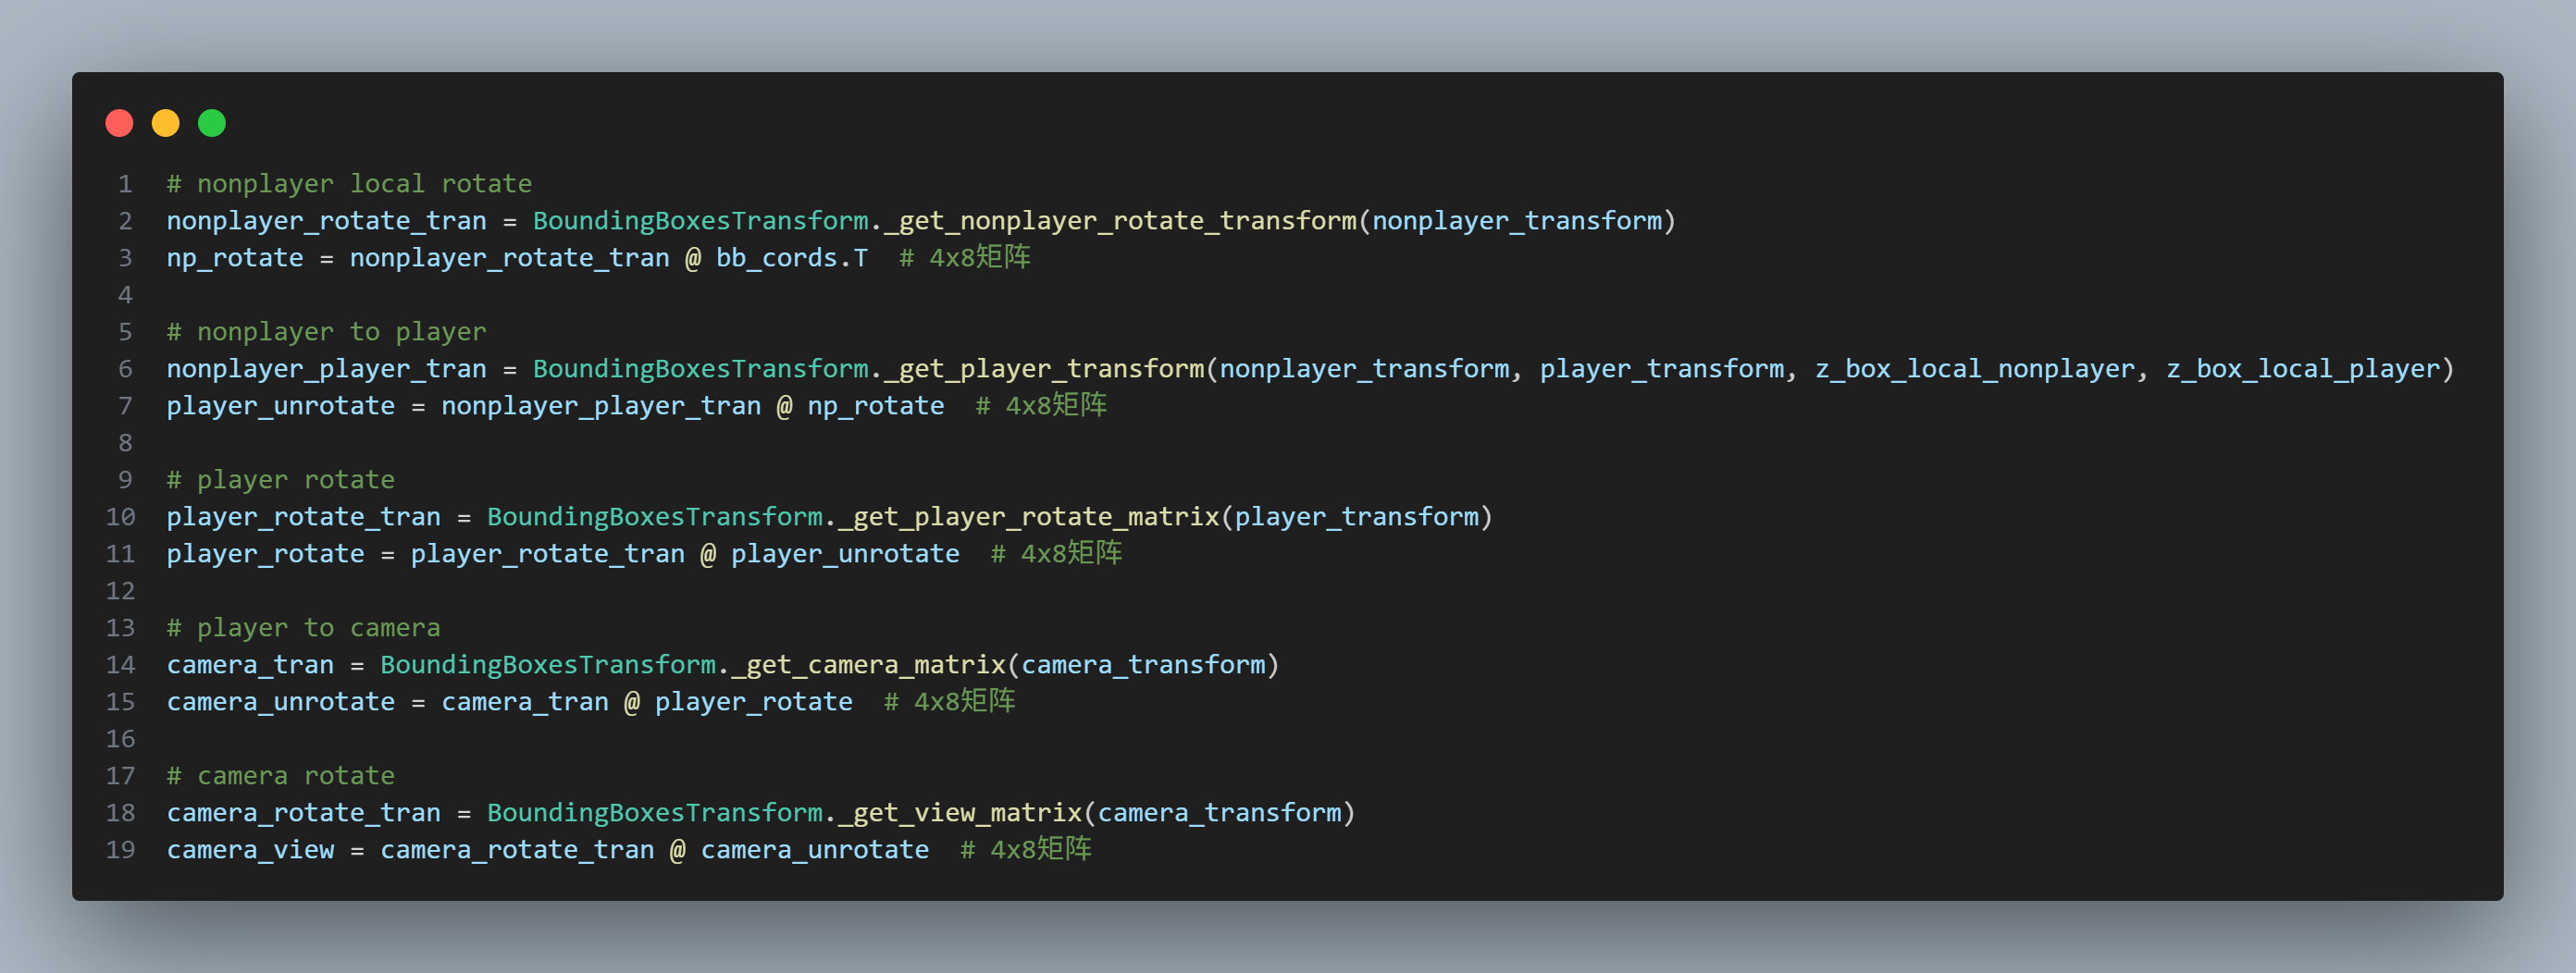
\includegraphics[width=1.0\textwidth]{pre1.png}
	\caption{}
	\label{fig:self_driving_keypoints}
\end{figure}
\begin{figure}[h]
	\centering
	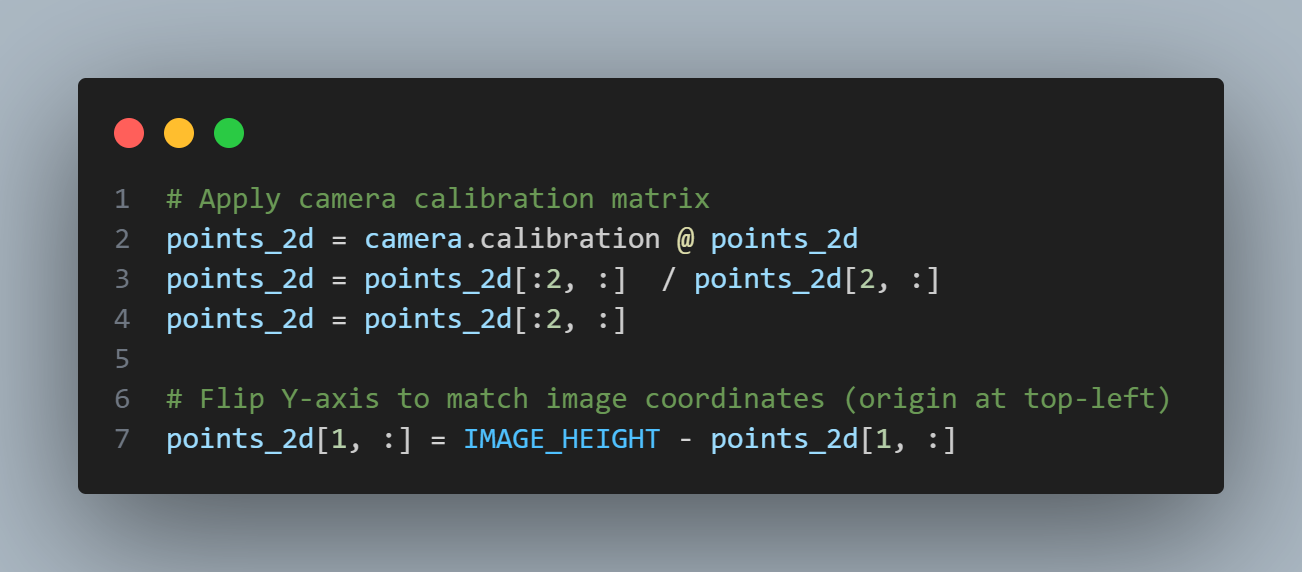
\includegraphics[width=0.5\textwidth]{pre2.png}
	\caption{}
	\label{fig:self_driving_3d_keypoints}
\end{figure}
\newpage
Here are the results of the self-driving detection algorithm: (3 figures)
\begin{figure}[h]
	\centering
	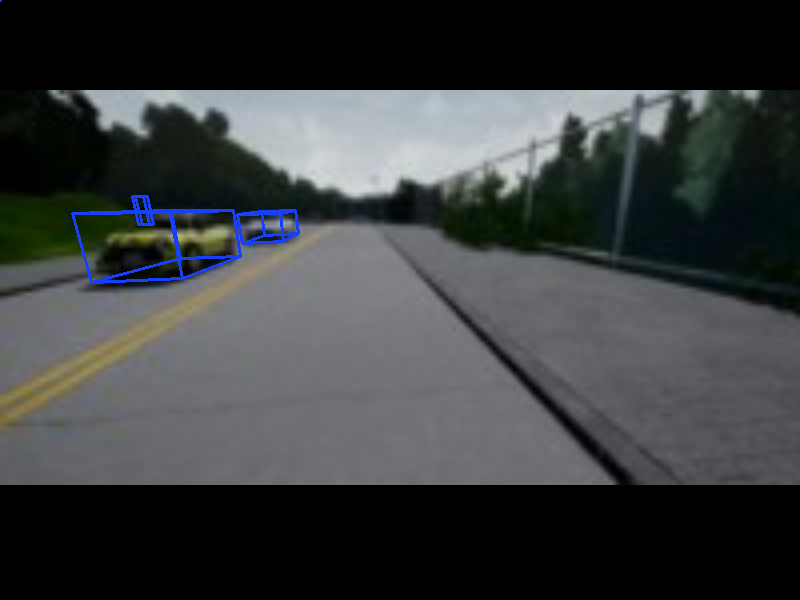
\includegraphics[width=0.5\textwidth]{src/problem3_driving/output/test_0.png}
	\caption{}
	\label{fig:self_driving_results_1}
\end{figure}
\begin{figure}[h]
	\centering
	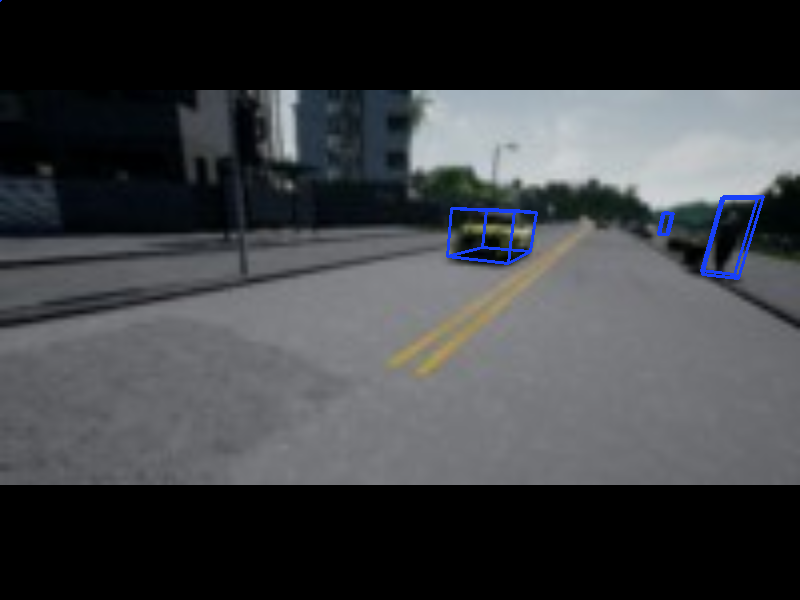
\includegraphics[width=0.5\textwidth]{src/problem3_driving/output/test_1.png}
	\caption{}
	\label{fig:self_driving_results_2}
\end{figure}
\begin{figure}[h]
	\centering
	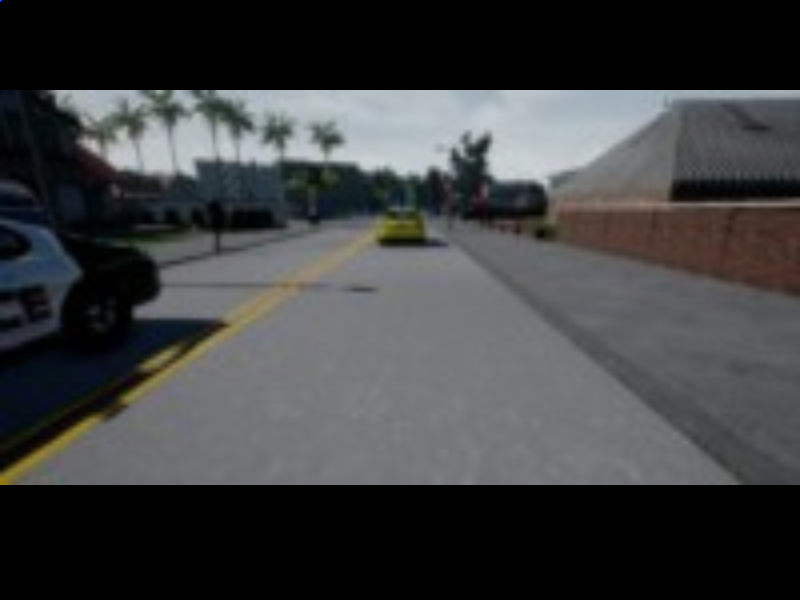
\includegraphics[width=0.5\textwidth]{src/problem3_driving/output/test_2.png}
	\caption{}
	\label{fig:self_driving_results_3}
\end{figure}

\end{document}